% -------------------------------------------
\mysec{Körper mit gekrümmten Flächen}\bigskip
% -------------------------------------------
Kugel:\medskip\par
\begin{minipage}{0.35\linewidth}
  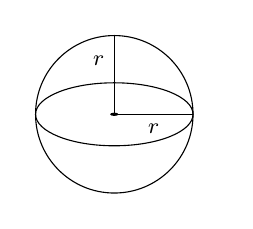
\begin{tikzpicture}
    \clip (-1.1, -1.1) rectangle (1.4, 1.1);
    \draw (0, 0) circle (1);
    \draw (0, 0) -- node[below]{{\footnotesize$r$}} (1, 0);
    \draw (0, 0) -- node[above left]{{\footnotesize$r$}} (0, 1);
    \fill (0, 0) ellipse (1.5pt and 0.6pt);
    \draw (0, 0) ellipse (1 and 0.4);
  \end{tikzpicture}%
\end{minipage}%
\begin{minipage}{0.65\linewidth}
  \formrow{O=4\pi r^{2}}
  \formrow{V=\frac{4}{3}\pi r^{3}}\vspace*{-\bigskipamount}
\end{minipage}\bigskip

Zylinder:\medskip\par
\begin{minipage}{0.35\linewidth}
  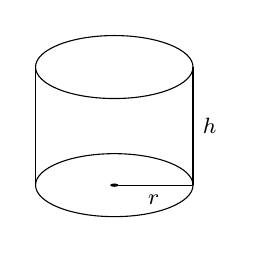
\begin{tikzpicture}
    \clip (-1.1, -0.5) rectangle (1.4, 2.0);
    \draw (-1, 0) -- (-1, 1.5);
    \draw (1, 0) -- node[right]{{\footnotesize$h$}} (1, 1.5);
    \draw (0, 1.5) ellipse (1 and 0.4);
    \draw (0, 0) ellipse (1 and 0.4);
    \draw (0, 0) -- node[below]{{\footnotesize$r$}} (1, 0);
    \fill (0, 0) ellipse (1.5pt and 0.6pt);
  \end{tikzpicture}%
\end{minipage}%
\begin{minipage}{0.65\linewidth}
  \formrow{O=2\pi r^{2}+2\pi rh}
  \formrow{V=\pi r^{2}h}\vspace*{-\bigskipamount}
\end{minipage}\bigskip

Kegel:\medskip\par
\begin{minipage}{0.35\linewidth}
  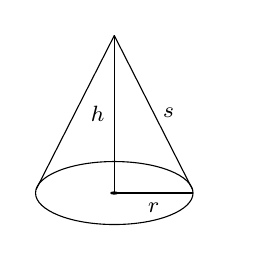
\begin{tikzpicture}
    \clip (-1.1, -0.5) rectangle (1.4, 2.1);
    \draw (0, 0) ellipse (1 and 0.4);
    \draw[cap=round] ([shift=(80:0.5mm)]-1, 0) -- (0, 2);
    \draw[cap=round] ([shift=(100:0.5mm)]1, 0) -- node[right]{{\footnotesize$s$}} (0, 2);
    \draw (0, 0) -- node[below]{{\footnotesize$r$}} (1, 0);
    \draw (0, 0) -- node[left]{{\footnotesize$h$}} (0, 2);
    \fill (0, 0) ellipse (1.5pt and 0.6pt);
  \end{tikzpicture}%
\end{minipage}%
\begin{minipage}{0.65\linewidth}
  \formrow{O=\pi r^{2}+\pi rs}
  \formrow{V=\frac{1}{3}\pi r^{2}h}\vspace*{-\bigskipamount}
\end{minipage}

